The Linear Kernel SVM had the worst performance in comparison to the others
SVMs. This fact can be seen in Table \ref{tab:linear_SVM}, in which is observed
that this machine does not classify any data point to the class 1 as the
sensitivity value is 0 for the three datasets.

\begin{table}
  \centering
  \caption{Performance scores for linear SVM.}
  \label{tab:linear_SVM}
  \begin{tabular}{ccc}
    \hline
    \textbf{Set} & \textbf{Sensitivity} & \textbf{Specificity} \\ \hline
    Training & 0 & 1 \\
    Testing & 0 & 1 \\
    Validation & 0 & 1 \\ \hline
  \end{tabular}
\end{table}

The fact that the Linear Kernel SVM could not learn the training data set shows
us, intuitively, that the data set is not linearly separable and that the data
set has some non-linearities that heavily difficult the learning of it.
Furthermore, in Fig. \ref{fig:SVM-linear} it is seen that in each of the
projections the decision function for the linear kernel SVM is always negative.

\begin{figure*}
  \centering
  \begin{subfigure}[b]{0.32\textwidth}
    \centering
    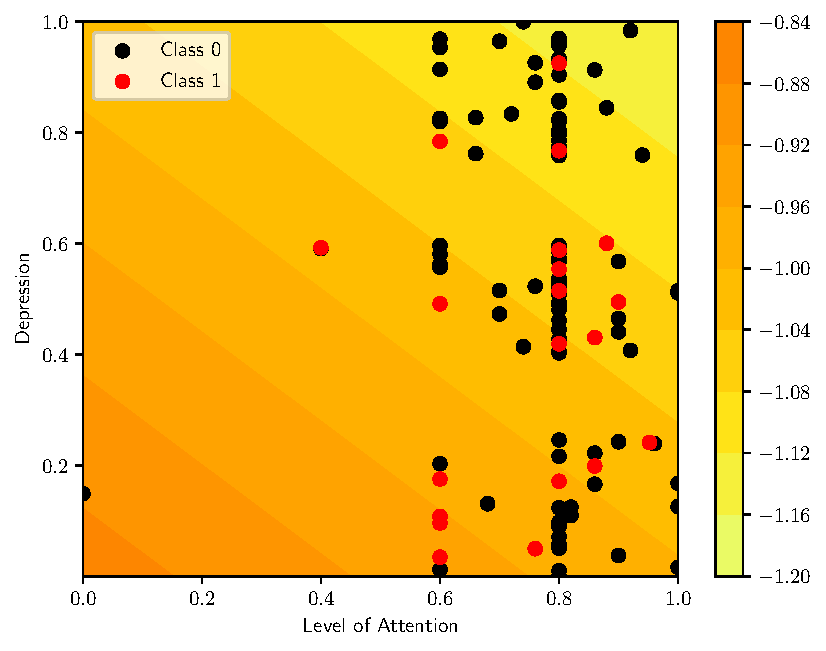
\includegraphics[width=\textwidth]{figs/svm-linear-contour-0-3.pdf}
    \caption{}
    \label{fig:SVM-linear1a}
  \end{subfigure}
  \begin{subfigure}[b]{0.32\textwidth}
    \centering
    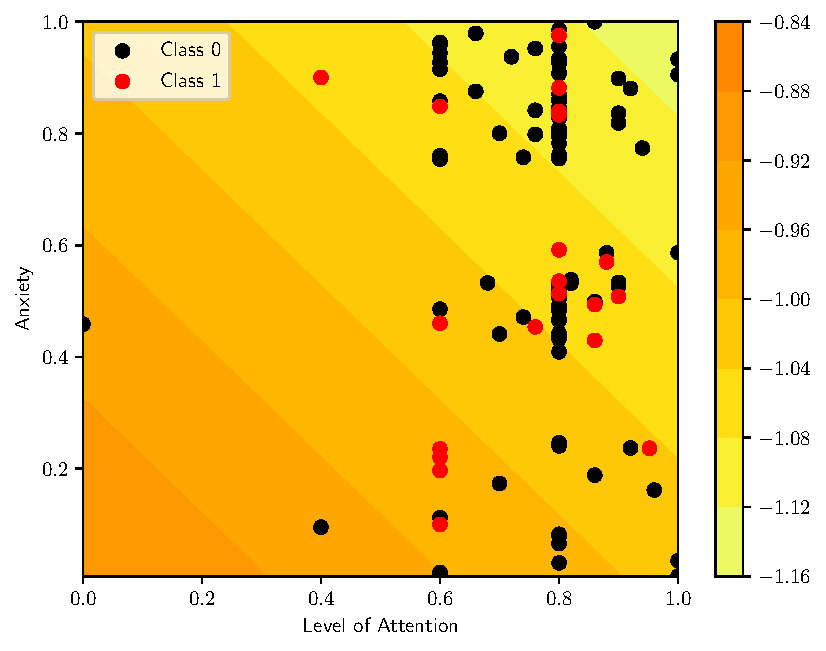
\includegraphics[width=\textwidth]{figs/svm-linear-contour-0-4.pdf}
    \caption{}
  \end{subfigure}
  \begin{subfigure}[b]{0.32\textwidth}
    \centering
    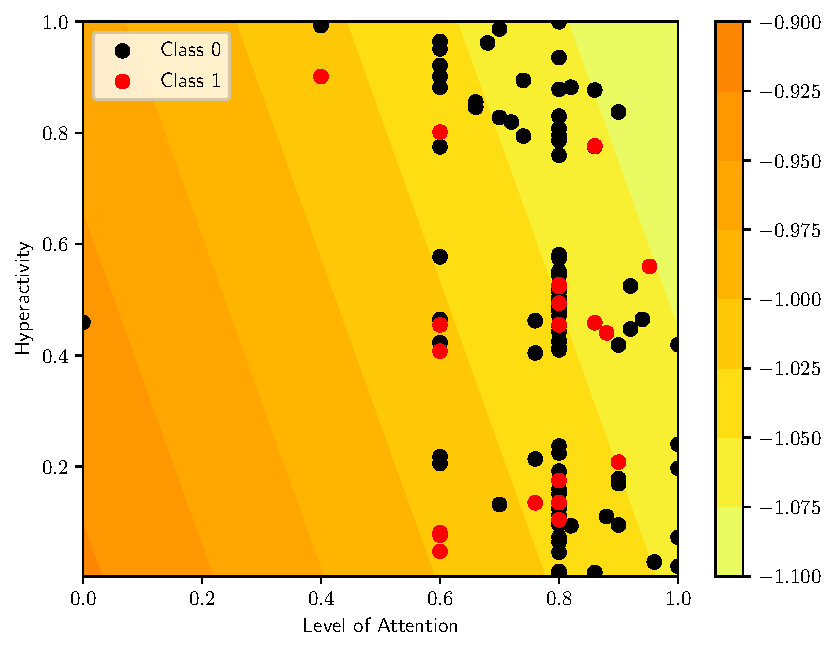
\includegraphics[width=\textwidth]{figs/svm-linear-contour-0-5.pdf}
    \caption{}
    \label{fig:SVM-linear1c}
  \end{subfigure}

  \begin{subfigure}[b]{0.32\textwidth}
    \centering
    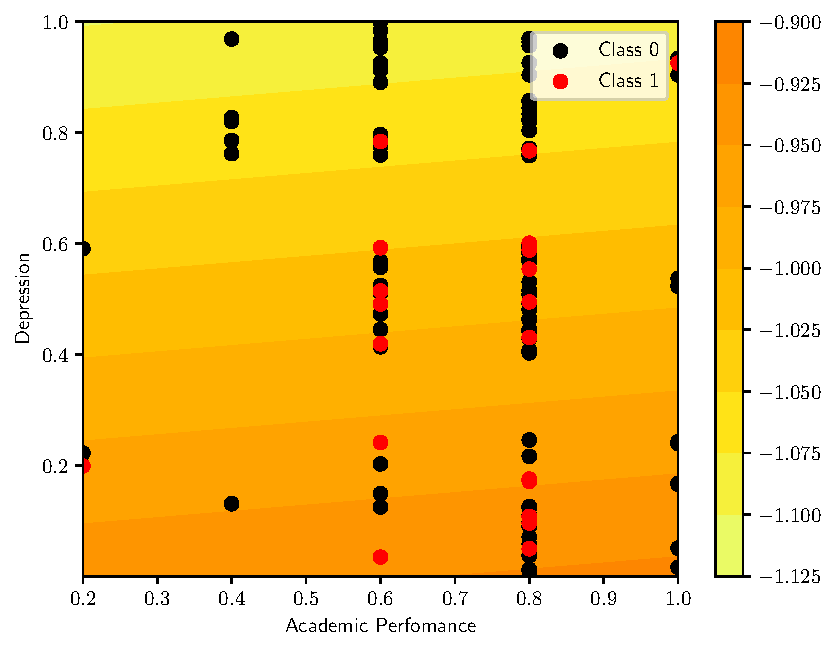
\includegraphics[width=\textwidth]{figs/svm-linear-contour-1-3.pdf}
    \caption{}
    \label{fig:SVM-linear2a}
  \end{subfigure}
  \begin{subfigure}[b]{0.32\textwidth}
    \centering
    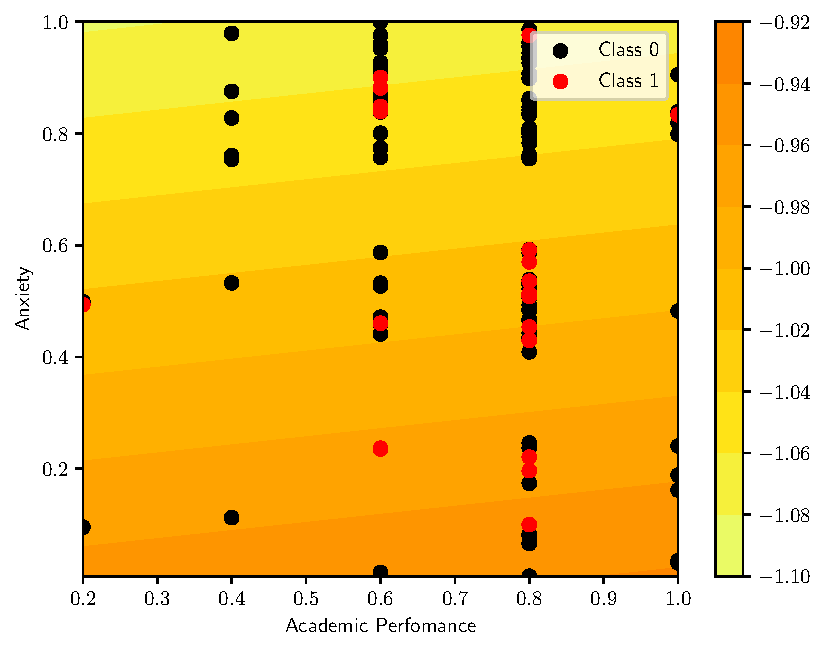
\includegraphics[width=\textwidth]{figs/svm-linear-contour-1-4.pdf}
    \caption{}
  \end{subfigure}
  \begin{subfigure}[b]{0.32\textwidth}
    \centering
    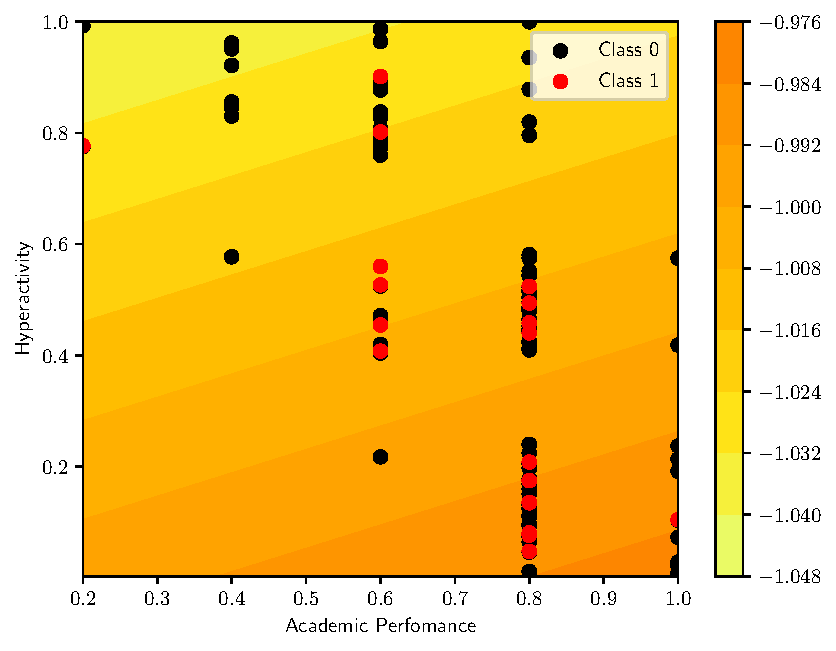
\includegraphics[width=\textwidth]{figs/svm-linear-contour-1-5.pdf}
    \caption{}
    \label{fig:SVM-linear2c}
  \end{subfigure}

  \begin{subfigure}[b]{0.32\textwidth}
    \centering
    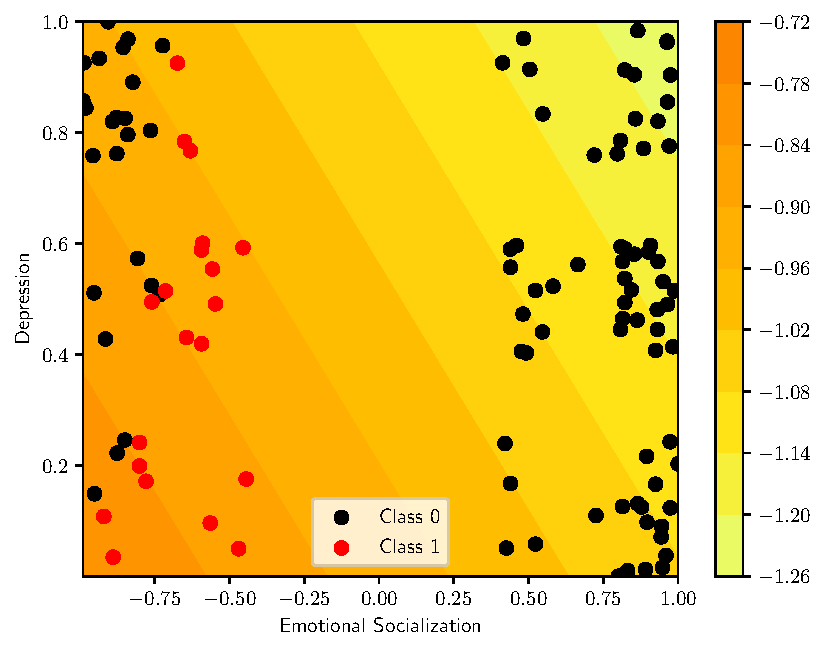
\includegraphics[width=\textwidth]{figs/svm-linear-contour-2-3.pdf}
    \caption{}
  \end{subfigure}
  \begin{subfigure}[b]{0.32\textwidth}
    \centering
    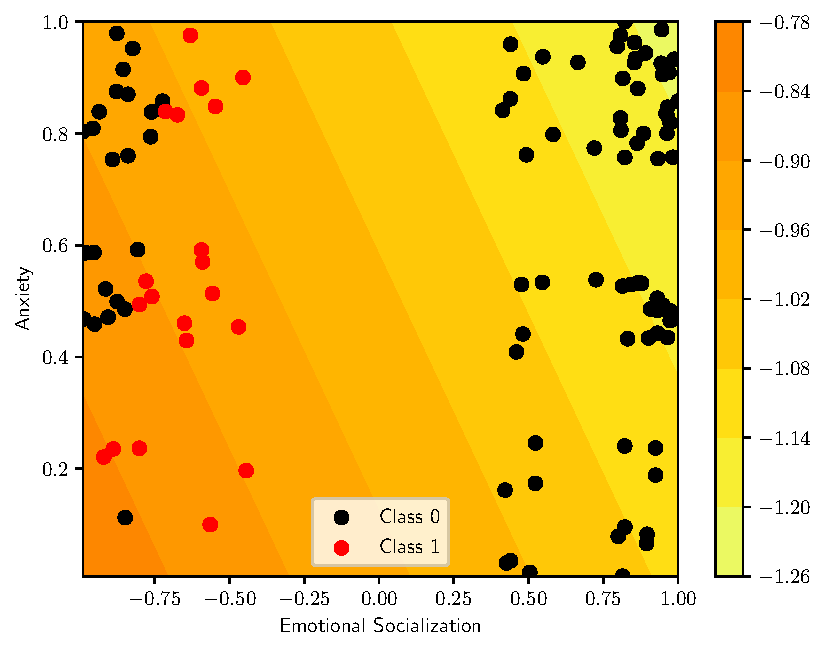
\includegraphics[width=\textwidth]{figs/svm-linear-contour-2-4.pdf}
    \caption{}
  \end{subfigure}
  \begin{subfigure}[b]{0.32\textwidth}
    \centering
    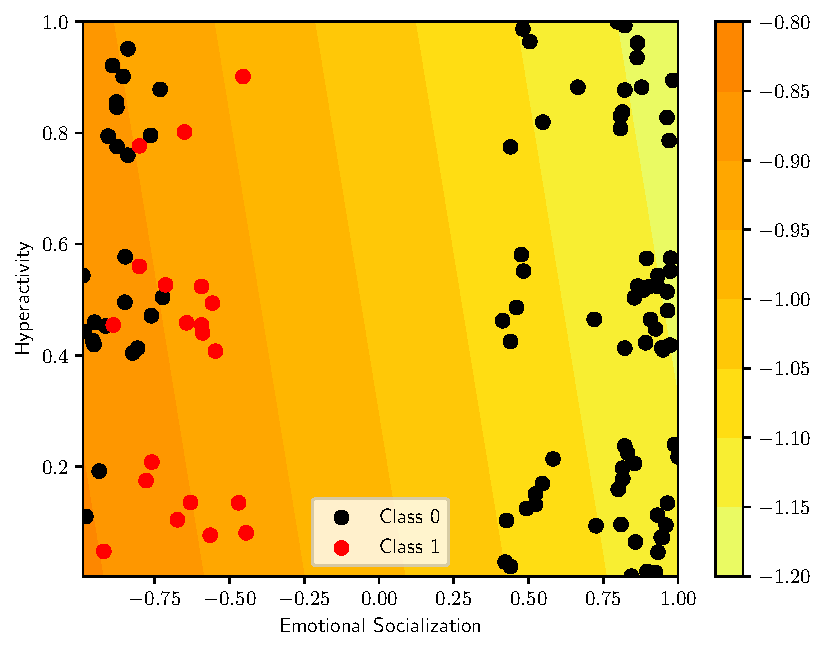
\includegraphics[width=\textwidth]{figs/svm-linear-contour-2-5.pdf}
    \caption{}
  \end{subfigure}
  \caption{Linear kernel SVM contour with real labels.}
  \label{fig:SVM-linear}
\end{figure*}

On the other hand, it is important to remark the contours still preserve a
linear structure. This fact assures us that the procedure for which these
contours are calculated can, partially, represent what's happening in higher
dimensions.

Lastly, it is also seen that in Figs.
\ref{fig:SVM-linear1a}-\ref{fig:SVM-linear1c},
\ref{fig:SVM-linear2a}-\ref{fig:SVM-linear2c} that the data are sparsed over
some discrete lines. This also verifies the realized projection as the variables
of this figures where measured as discrete variables in the used survey.

The Polynomial Kernel SVM had the best performance in the SVM category,
reflected in Table \ref{tab:poly_SVM}. One important thing to notice is that the
machine, as well as the RBF kernel SVM, was able to learn the class 0 for all
the datasets. This fact shows that the dynamic of class 0 is easier to
generalize and, probably, is linearly separable from class 1.

\begin{table}
  \centering
  \caption{Performance scores for polynomial SVM.}
  \label{tab:poly_SVM}
  \begin{tabular}{cll}
    \hline
    \textbf{Set} & \multicolumn{1}{c}{\textbf{Sensitivity}} & \multicolumn{1}{c}{\textbf{Specificity}} \\ \hline
    Training & 0.89 & 1 \\
    Testing & 0 & 1 \\
    Validation & 0.57 & 1 \\ \hline
  \end{tabular}
\end{table}

On the other hand, as shown by Figs. \ref{fig:SVM-poly3a}-\ref{fig:SVM-poly3c},
it is seen that class 0 is detailed (mostly) by the points in the middle of the
graph. This underlies a problem in classifying these data points as they do not
present any drastic behavior. In this manner, this SVM was able to classify it
with some precision and shows that more data are required to fully train the
machine to learn class 1.

\begin{figure*}
  \centering
  \begin{subfigure}[b]{0.32\textwidth}
    \centering 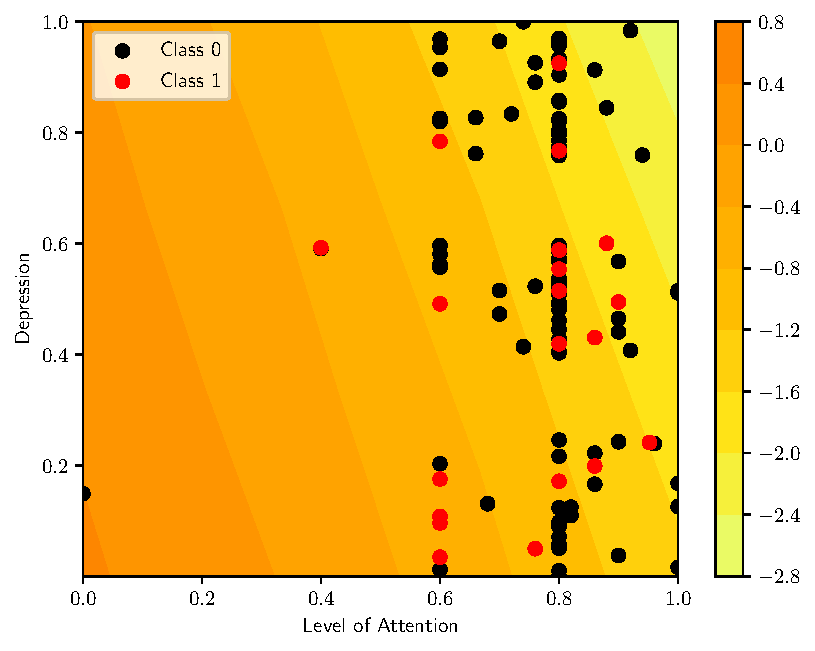
\includegraphics[width=\textwidth]{figs/svm-poly-contour-0-3.pdf}
    \caption{}
    \label{fig:SVM-poly1a}
  \end{subfigure}
  \begin{subfigure}[b]{0.32\textwidth}
    \centering 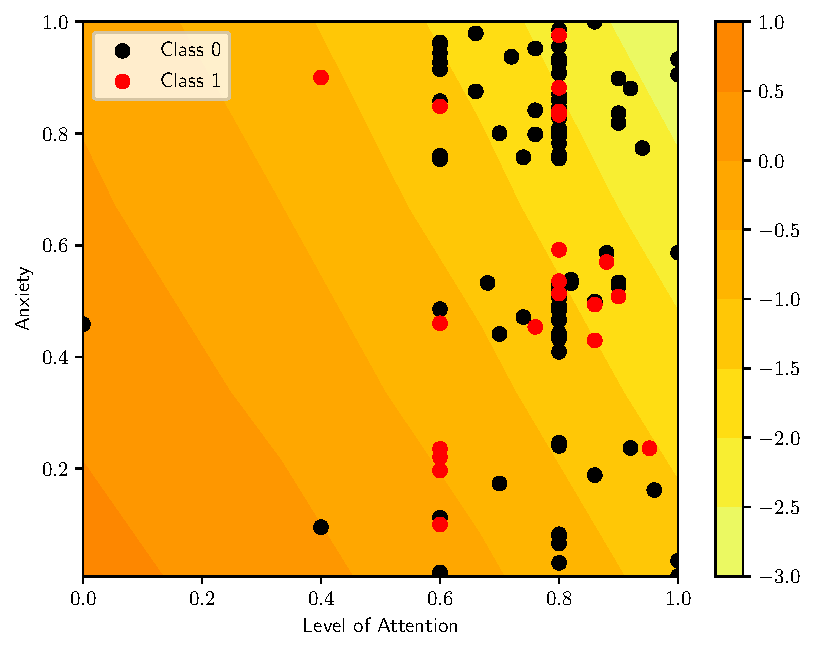
\includegraphics[width=\textwidth]{figs/svm-poly-contour-0-4.pdf}
    \caption{}
  \end{subfigure}
  \begin{subfigure}[b]{0.32\textwidth}
    \centering 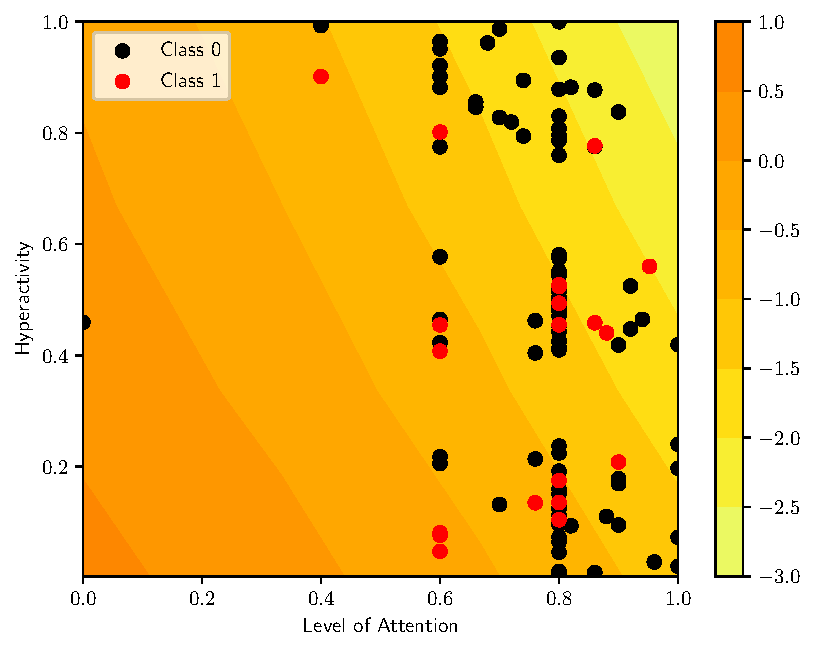
\includegraphics[width=\textwidth]{figs/svm-poly-contour-0-5.pdf}
    \caption{}
    \label{fig:SVM-poly1c}
  \end{subfigure}

  \begin{subfigure}[b]{0.32\textwidth}
    \centering 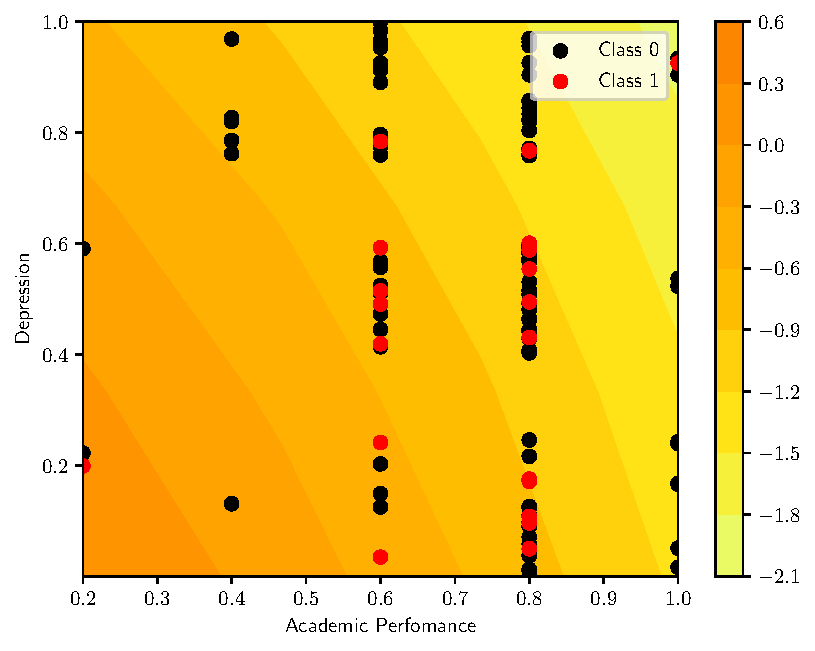
\includegraphics[width=\textwidth]{figs/svm-poly-contour-1-3.pdf}
    \caption{}
    \label{fig:SVM-poly2a}
  \end{subfigure}
  \begin{subfigure}[b]{0.32\textwidth}
    \centering 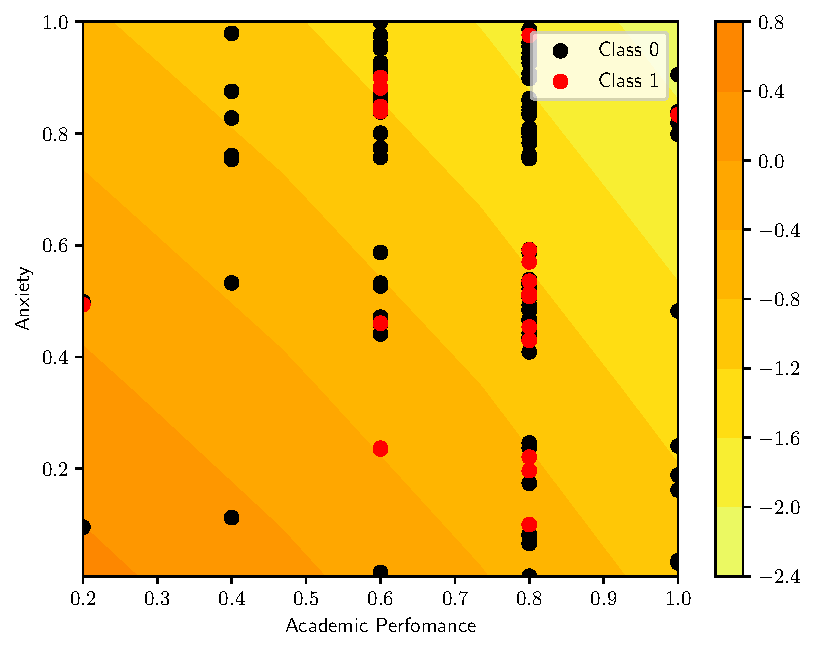
\includegraphics[width=\textwidth]{figs/svm-poly-contour-1-4.pdf}
    \caption{}
  \end{subfigure}
  \begin{subfigure}[b]{0.32\textwidth}
    \centering 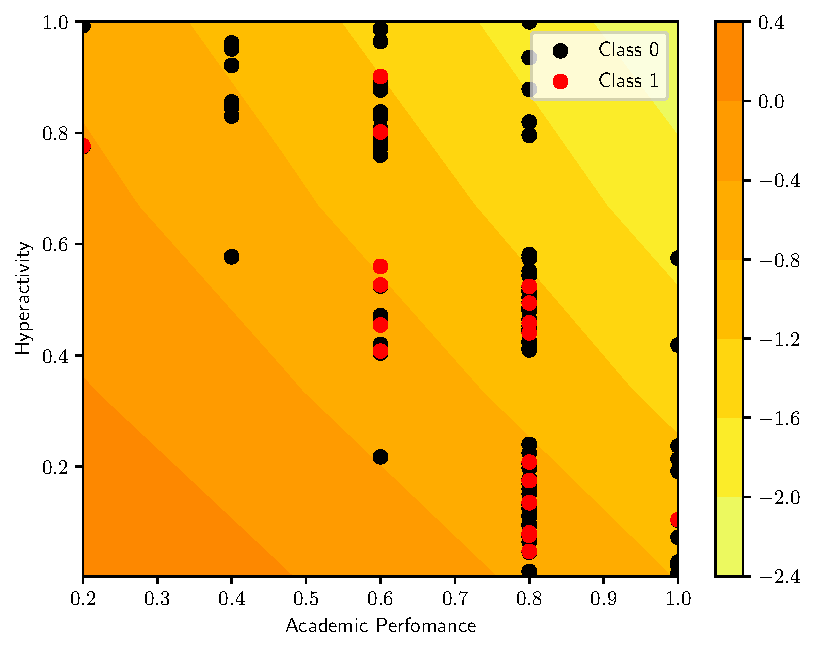
\includegraphics[width=\textwidth]{figs/svm-poly-contour-1-5.pdf}
    \caption{}
    \label{fig:SVM-poly2c}
  \end{subfigure}

  \begin{subfigure}[b]{0.32\textwidth}
    \centering 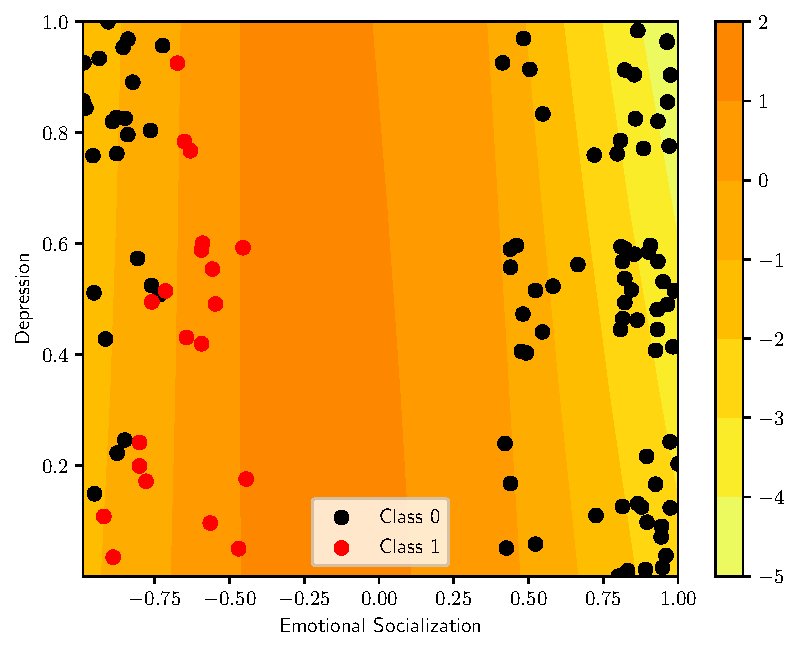
\includegraphics[width=\textwidth]{figs/svm-poly-contour-2-3.pdf}
    \caption{}
    \label{fig:SVM-poly3a}
  \end{subfigure}
  \begin{subfigure}[b]{0.32\textwidth}
    \centering 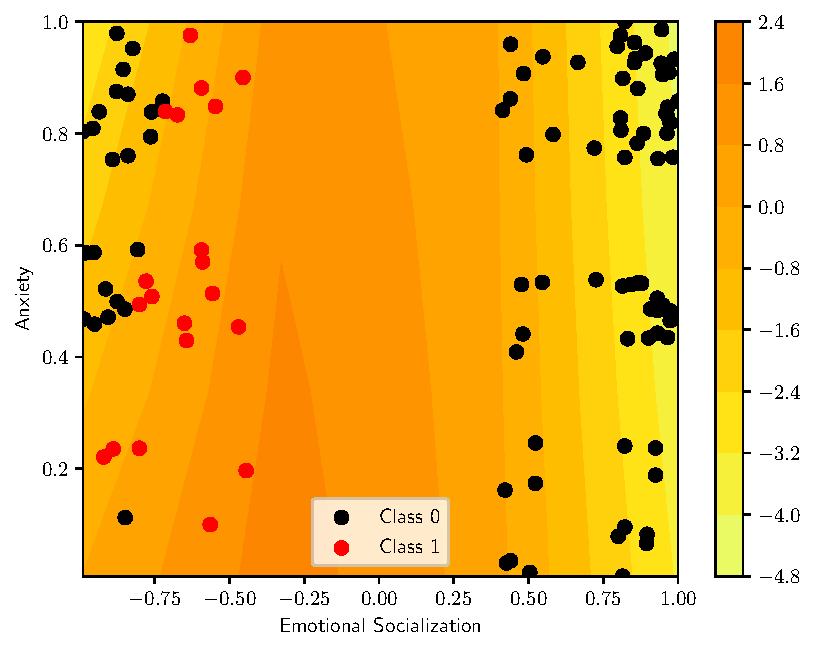
\includegraphics[width=\textwidth]{figs/svm-poly-contour-2-4.pdf}
    \caption{}
  \end{subfigure}
  \begin{subfigure}[b]{0.32\textwidth}
    \centering 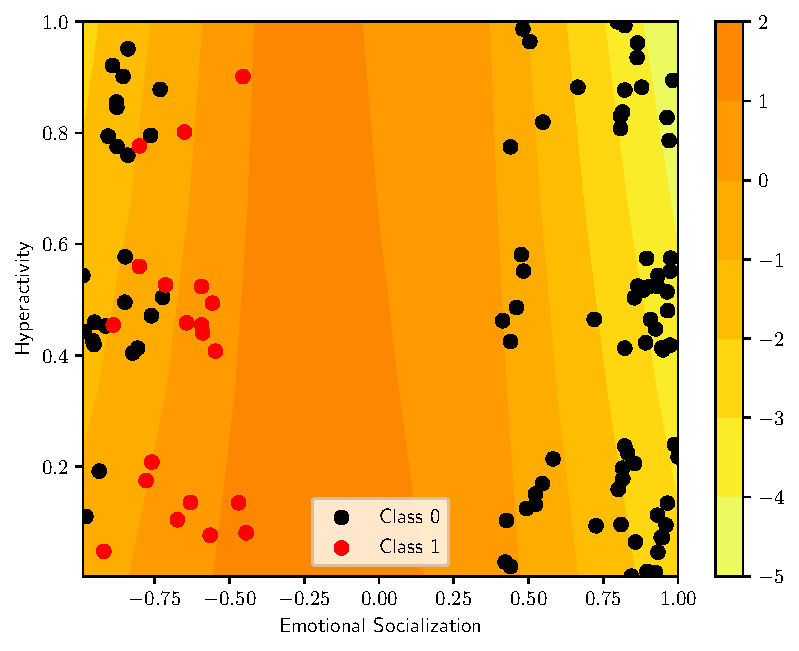
\includegraphics[width=\textwidth]{figs/svm-poly-contour-2-5.pdf}
    \caption{}
    \label{fig:SVM-poly3c}
  \end{subfigure}
  \caption{Polynomial kernel SVM contour with real labels.}
  \label{fig:SVM-poly}
\end{figure*}

Lastly, it is seen that Figs. \ref{fig:SVM-poly1a}-\ref{fig:SVM-poly1c},
\ref{fig:SVM-poly2a}-\ref{fig:SVM-poly2c} are not critical in separating the
data. This occurs because the independent variable in these plots is discrete
and probably does not contain much information surrounding the problem. This
will be also be highlighted by the decision tree.

The RBF kernel SVM had the second-best performance, as at least it was able to
recognize some of the data from class 1 (in comparison to the Linear SVM). This
is expected as in each of the projections the data did not present any circular
relationship. This issue with using an RBF kernel can be visualized in Fig.
\ref{fig:svm-rbf}.

It is important to note, that, as with all the SVMs, the contour plotted
preserves the structure of the used kernel and therefore confirms that the
procedure used is correct.

\begin{figure*}
  \centering
  \begin{subfigure}[b]{0.32\textwidth}
    \centering 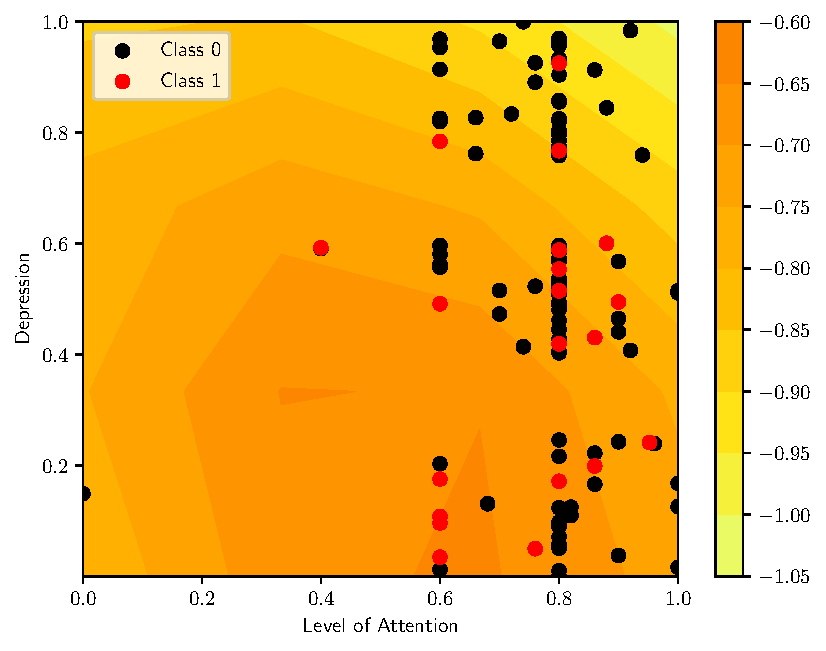
\includegraphics[width=\textwidth]{figs/svm-rbf-contour-0-3.pdf}
    \caption{}
  \end{subfigure}
  \begin{subfigure}[b]{0.32\textwidth}
    \centering 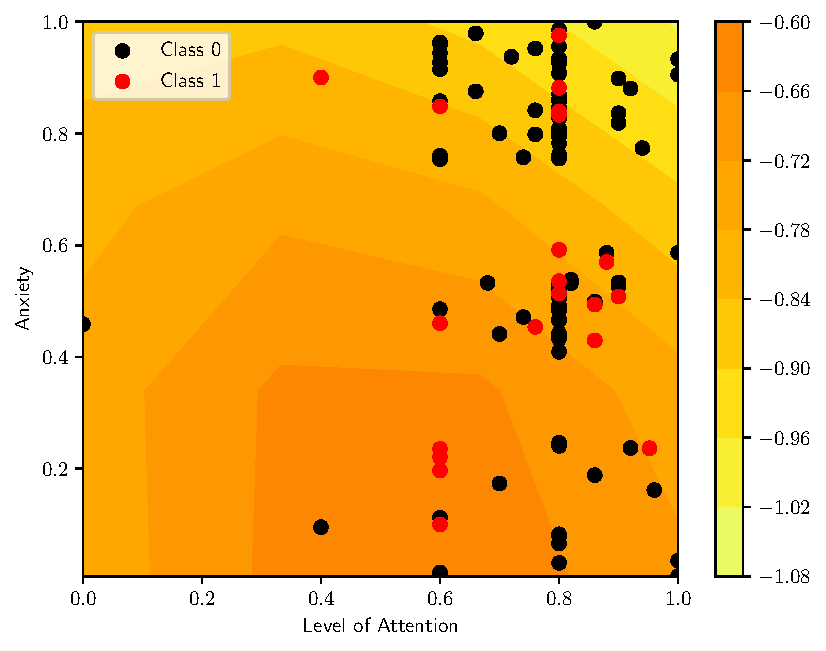
\includegraphics[width=\textwidth]{figs/svm-rbf-contour-0-4.pdf}
    \caption{}
  \end{subfigure}
  \begin{subfigure}[b]{0.32\textwidth}
    \centering 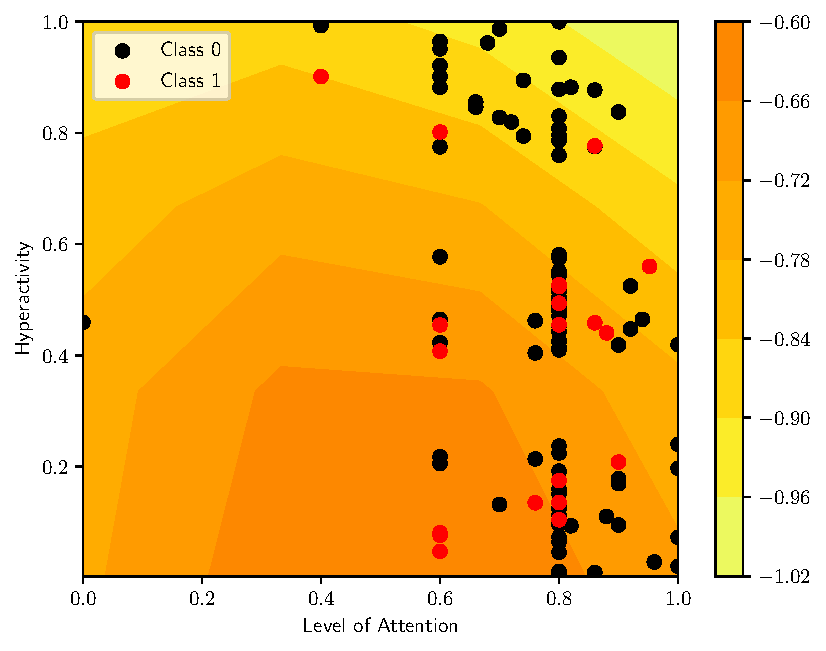
\includegraphics[width=\textwidth]{figs/svm-rbf-contour-0-5.pdf}
    \caption{}
  \end{subfigure}

  \begin{subfigure}[b]{0.32\textwidth}
    \centering 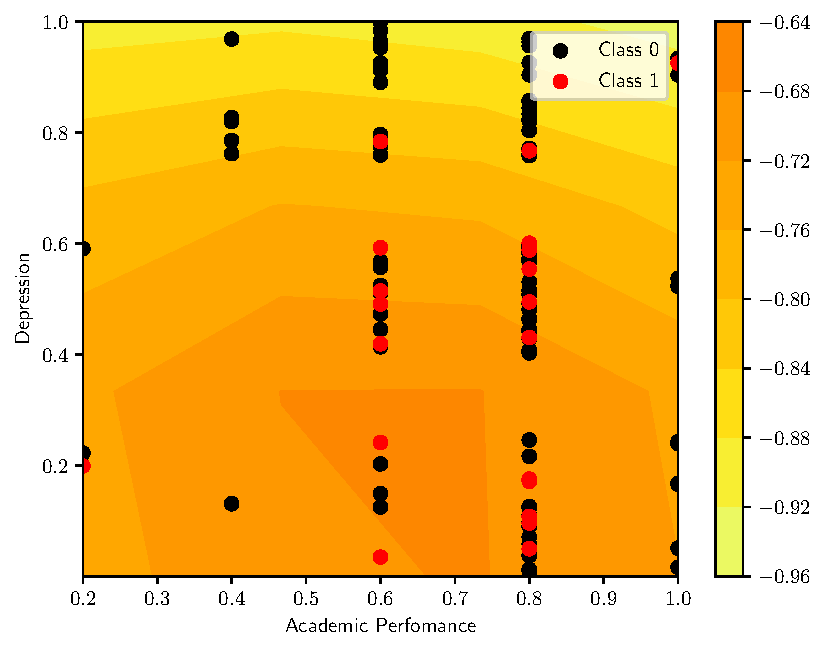
\includegraphics[width=\textwidth]{figs/svm-rbf-contour-1-3.pdf}
    \caption{}
  \end{subfigure}
  \begin{subfigure}[b]{0.32\textwidth}
    \centering 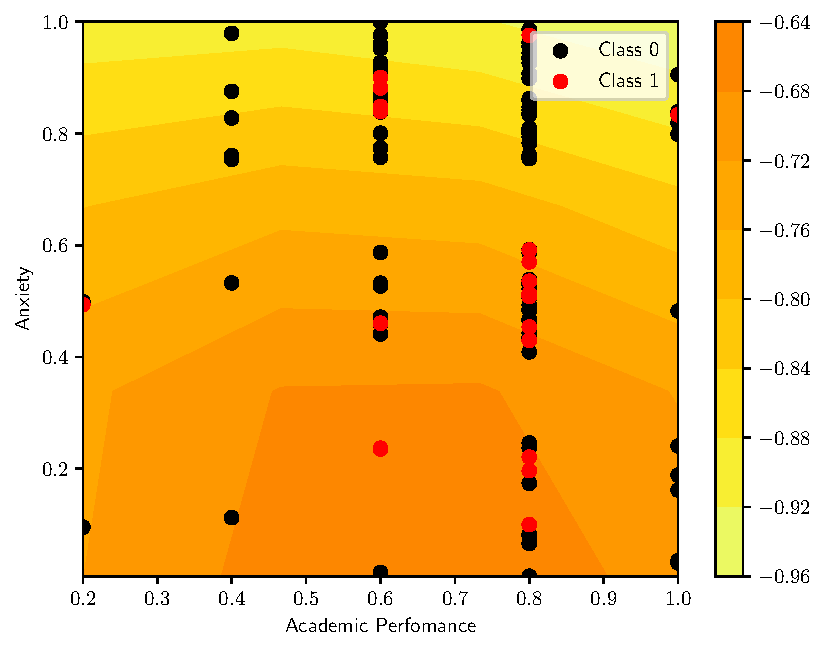
\includegraphics[width=\textwidth]{figs/svm-rbf-contour-1-4.pdf}
    \caption{}
  \end{subfigure}
  \begin{subfigure}[b]{0.32\textwidth}
    \centering 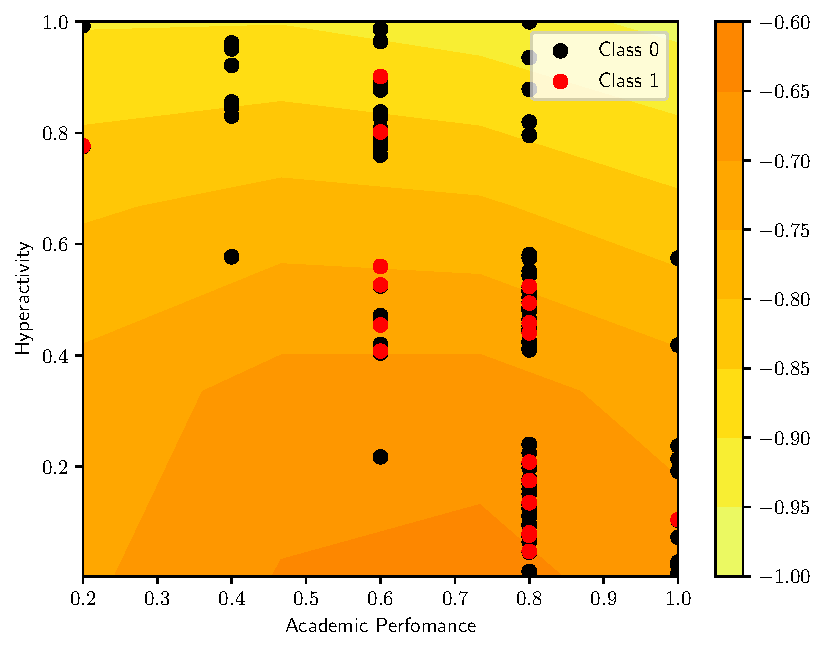
\includegraphics[width=\textwidth]{figs/svm-rbf-contour-1-5.pdf}
    \caption{}
  \end{subfigure}

  \begin{subfigure}[b]{0.32\textwidth}
    \centering 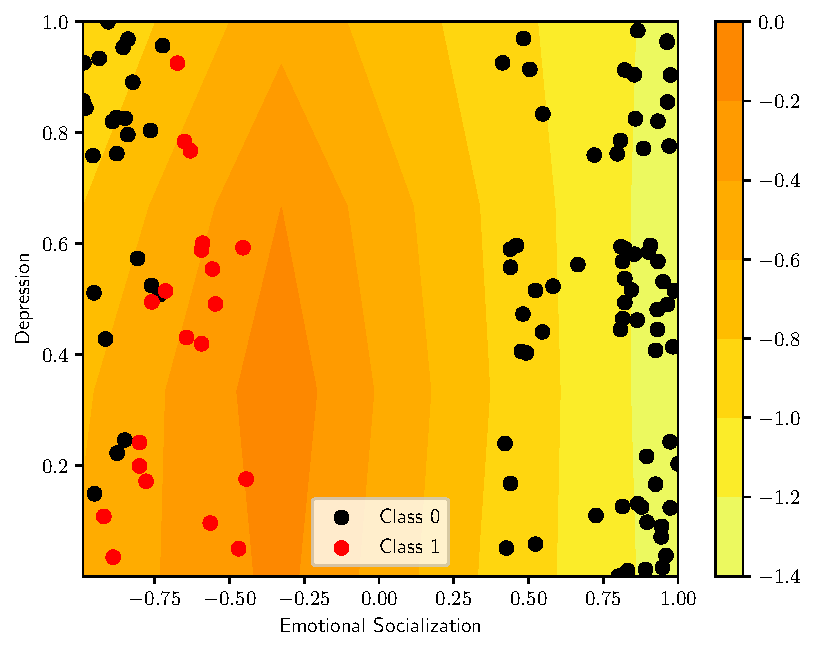
\includegraphics[width=\textwidth]{figs/svm-rbf-contour-2-3.pdf}
    \caption{}
  \end{subfigure}
  \begin{subfigure}[b]{0.32\textwidth}
    \centering 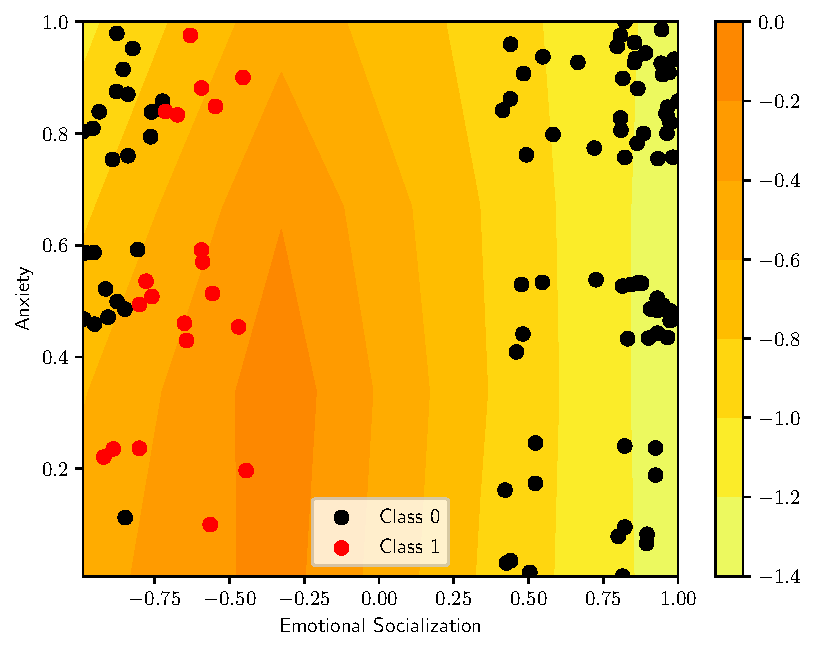
\includegraphics[width=\textwidth]{figs/svm-rbf-contour-2-4.pdf}
    \caption{}
  \end{subfigure}
  \begin{subfigure}[b]{0.32\textwidth}
    \centering 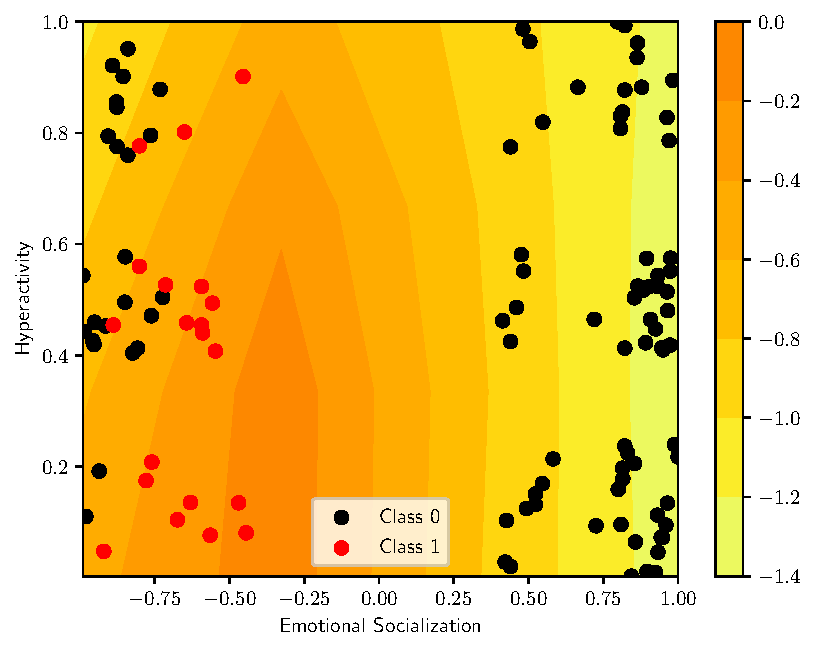
\includegraphics[width=\textwidth]{figs/svm-rbf-contour-2-5.pdf}
    \caption{}
  \end{subfigure}
  \caption{RBF kernel SVM contour with real labels.}
  \label{fig:SVM-rbf}
\end{figure*}

\begin{table}
  \centering
  \caption{Performance scores for RBF SVM.}
  \label{tab:rbf_SVM}
  \begin{tabular}{cll}
    \hline
    \textbf{Set} & \multicolumn{1}{c}{\textbf{Sensitivity}} & \multicolumn{1}{c}{\textbf{Specificity}} \\ \hline
    Training & 0.13 & 1 \\
    Testing & 0 & 1 \\
    Validation & 0.25 & 1 \\ \hline
  \end{tabular}
\end{table}
